\begin{blocksection}
\question Draw the environment diagram that results from running the following code.

\begin{lstlisting}
def funny(joke):
    hoax = joke + 1
    return funny(hoax)

def sad(joke):
    hoax = joke - 1
    return hoax + hoax

funny, sad = sad, funny
result = funny(sad(2))
\end{lstlisting}
\begin{solution}[2in]
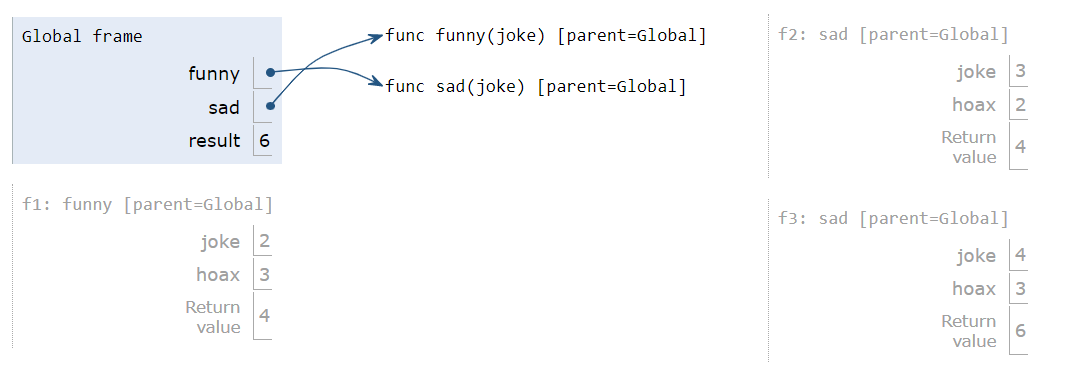
\includegraphics[scale=0.5]{joke.png}
\\
\url{https://tinyurl.com/y5lc4fez}
\end{solution}
\end{blocksection}

\begin{questionmeta}
    \textbf{Teaching Tips}
      \begin{itemize}
        \item Some students might have done swaps in other languages, but make sure to make the distiction as to why \lstinline{funny, sad = sad, funny} works in Python
        \item evaluate the functions on the RHS first, then assign to variables on the LHS
        \item Make sure that the students understand how Python looks for a value of a variable, from local (to parent(s)) to global
      \end{itemize}
    \end{questionmeta}
    